\section{Introduction}

%%%%%\begin{executivesummary}
%The executive summary should provide more background and context over
% and above the abstract, and also
% possibly include a road-map to the document.
%Section \ref{foo}: ...

The Combine system is an open, free, and highly configurable
system for focused crawling of Internet resources.
It aims at providing a robust and efficient tool for creating
topic-specific moderate sized databases (up to a few million records).
Crawling speed is around 200 URLs per minute and a complete structured
record takes up an average of 25 kilobytes disk-space.

\begin{figure}[htb]
\begin{center}
 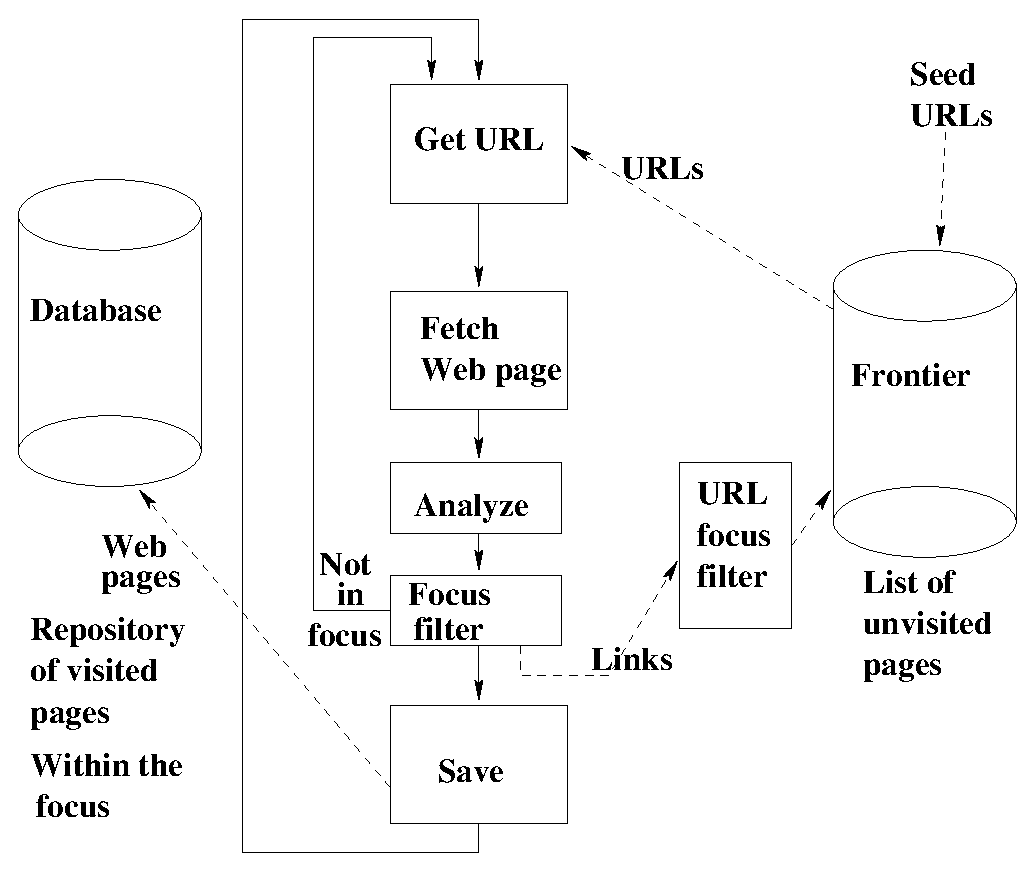
\includegraphics[height=0.3\textheight, width=0.6\textwidth]{focusedrobot.eps}
\end{center}
\caption{Overview of the Combine focused crawler.}
\label{overview}
\end{figure}

\hspace{-\parindent}Main features include:
\begin{itemize}
\item part of the \htmladdnormallinkfoot{SearchEngine-in-a-Box}{http://combine.it.lth.se/SearchEngineBox/} system
\item extensive configuration possibilities
\item integrated topic filter (automated topic classifier) for focused crawling mode
\item possibility to use any topic filter (if provided as a \htmladdnormallinkfoot{Perl Plug-In module}{http://combine.it.lth.se/PlugIns/}) in focused crawling mode
\item crawl limitations based on regular expression on URLs -
both include and exclude rules (URL focus filter)
\item character set detection/normalization
\item language detection
\item HTML cleaning
\item metadata extraction
\item duplicate detection
\item HTML parsing to provide structured records for each crawled page
\item support for many document formats (text, HTML, PDF, PostScript, MSWord, MSPowerPoint, MSExcel, RTF, TeX, images)
\item SQL database for data storage and administration
\end{itemize}

Naturally it obeys the \htmladdnormallinkfoot{Robots
  Exclusion Protocol}{http://www.robotstxt.org/wc/exclusion.html}
and behaves nice to Web-servers. Besides focused crawls (generating
topic-specific databases), Combine supports configurable rules on
what's crawled based on regular expressions on URLs (URL focus filter).
The crawler is designed to run continuously in order to keep
crawled databases as up to date as possible. It can be stopped and
restarted any time without loosing any status or information.

The operation of Combine (overview in Figure \ref{overview}) as a focused crawler is based on a combination of a
general Web crawler and an automated subject classifier. The topic
focus is provided by a focus filter using a topic
definition implemented as a thesaurus, where each term is connected to a
topic class.

Crawled data are stored as a
structured records in a local relational database.

%%%%%%%%%%%%%%%%
Section \ref{distr}
 outlines how to download, install and test the Combine system and includes use scenarios -- useful in order to get a jump start at using the system.

Section \ref{configuration} discusses configuration structure and highlights a few important configuration variables.

Section \ref{operation} describes policies and methods used by the crawler.

 Evaluation and performance are treated in sections
\ref{autoclasseval} and \ref{performance}.

%%%%\end{executivesummary}

The system has a number of \hyperref{components}{components (see
section }{)}{comp}, the main ones visible to the user being {\tt combineCtrl}
which is used to start and stop crawling and view crawler status, and
{\tt combineExport} that extracts crawled data from the internal
database and exports them as XML records.

Further details (lots and lots of them) can be found in \hyperref{'Gory details'}{part }{ 'Gory details'}{gory} and in \hyperref{the Appendix}{Appendix }{}{appendix}.
